\documentclass[12pt,a4paper]{article}
\usepackage[utf8]{inputenc}
\usepackage{amsmath}
\usepackage[labelfont=bf]{caption}
\usepackage{amsfonts}
\usepackage{amssymb}
\usepackage{graphicx}
\usepackage{fourier}
\usepackage[left=3cm,right=3cm,top=3cm,bottom=3cm]{geometry}
\author{Devin Cody}
\title{An Introduction to Radio Interferometry for Engineers}
\begin{document}

\maketitle

\section{Introductions}

Hi! Welcome to my blog. As this is my first post, I thought I’d give a quick introduction of myself before we delve into my introduction of interferometry. My name is Devin and I’m currently a graduate student at Caltech studying towards a Master’s degree in Electrical Engineering. My primary interest is instrumentation. My passion is building hardware systems that allow us to better understand the world around us (e.g. Radio telescopes, Quantum Circuits, Rockets). However, a lot of the work that I’ve done has been bringing these types of systems to life through software development, so I consider myself a bit of a mixed bag of skills and expertise.  If you’re interested in learning more about what I do or how I do it, please check out my website at devincody.com

Currently at Caltech, I’m working with Gregg Hallinan and Sandy Weinreb on a project called the Long Wavelength Array (LWA). The LWA is a 256-element interferometer in Owens Valley, CA which takes radio images of the entire sky every 10 seconds. This project is particularly exciting for me because I’ve always been interested in how many distinct dishes can synthesize coherent images, sometimes with resolutions that cannot be achieved with single dish telescopes!

Radio interferometry often times comes off as a difficult concept, but it doesn’t need to be that way. In this blog post, I will attempt to give a more intuitive introduction to radio interferometry, one that, in particular, might help a budding radio engineer learn more about this fascinating field. I will assume knowledge of calculus, but everything else will be developed from the ground up. 

	
\section{Starting with the Punchline}
	
  In this blog post, I will start with the big punchline of radio interferometry and then work backwards to then justify everything else. So, are you ready for it? The big reveal? Ok, here it is: the most mind-blowing fact about radio astronomy is that instead of directly observing the sky, radio interferometers measure the Fourier transform of the sky. Slow down, don’t leave just yet, let’s take a minute to break this down. The Fourier transform is a method of taking a sequence of data which is represented in one way (i.e. a series of measurements over time, a signal coming from a sensor, or series of pixels across a spatial grid[\^1]) and representing it in a different, but equally valid way. When you take the Fourier transform of some data, no information is lost. The data has simply been rearranged. Simultaneously, there exists a method by which we can take some data which has been Fourier transformed and undo the Fourier transform to recover the original data. This procedure is called the inverse Fourier transform. The important thing to take away from this, is that if we measure the Fourier transform of the sky, then we can reconstruct an map (image) of the sky brightness by taking the inverse Fourier transform of that data. But enough words, let’s look at some pictures.

\begin{figure}
\centering
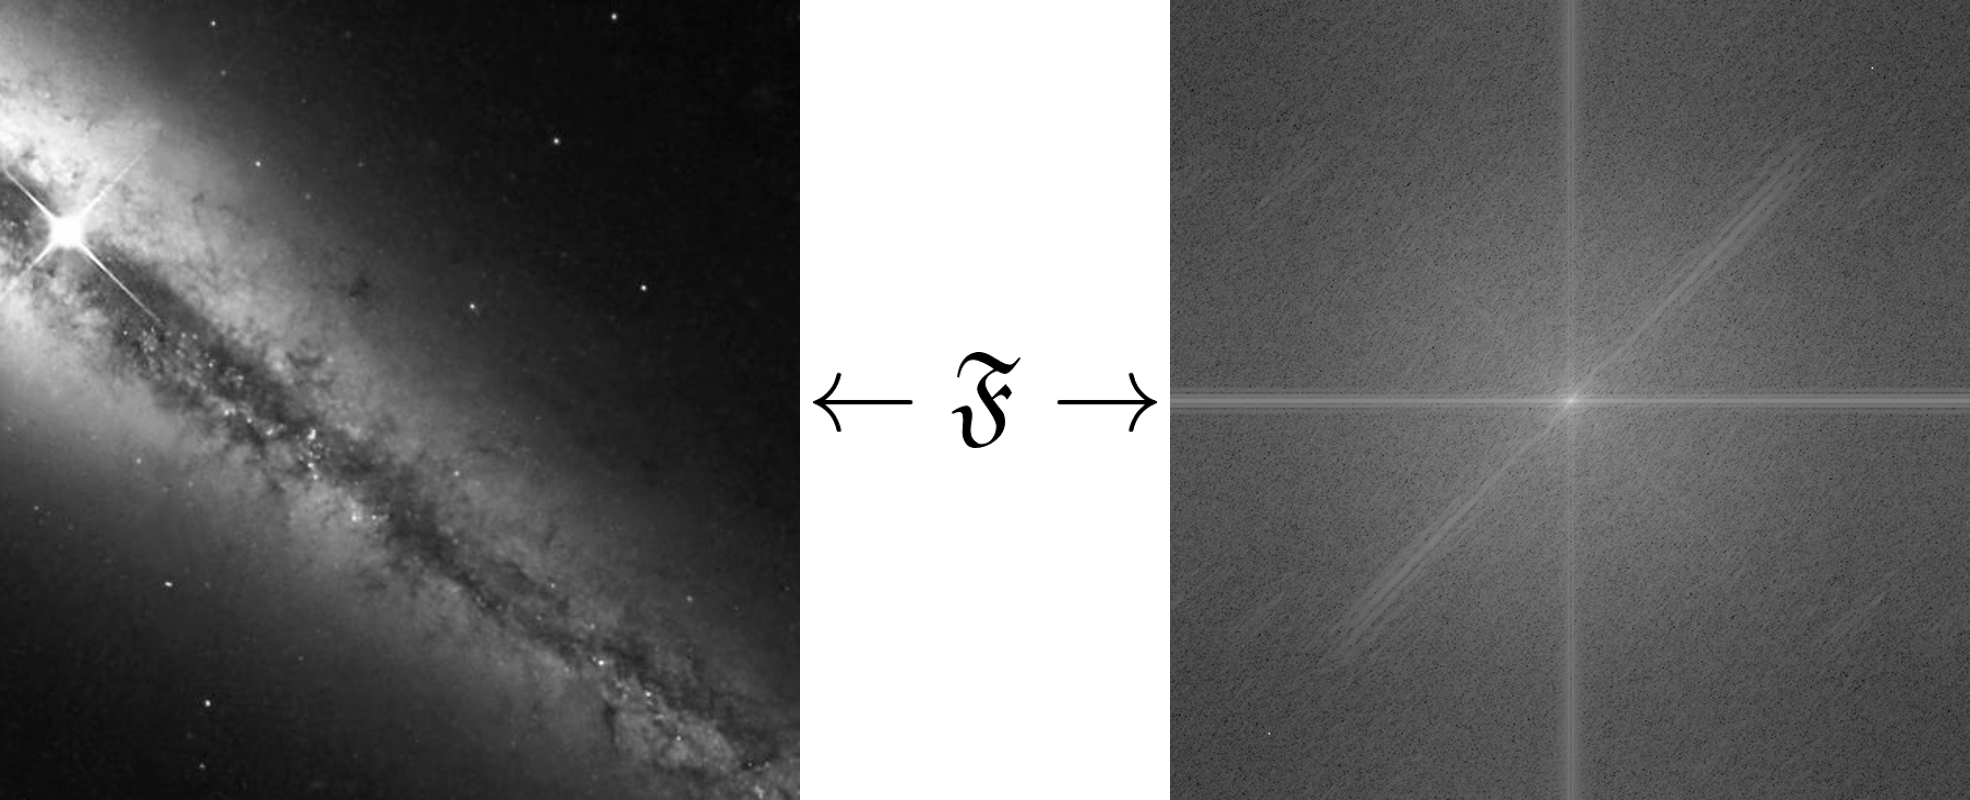
\includegraphics[width=\textwidth]{_images/FT.png}
\caption{\textbf{Galaxy in \textit{Image} Domain (left) and \textit{Fourier} Domain (right) |} Comparison of the ``traditional'' depiction of a galaxy in the \textit{image} domain (Left) and an equally-valid depiction of the same galaxy in \textit{Fourier} domain (Right). The script F denotes that these two images are related by the Fourier Transform.}
\end{figure}

Fig. 1 shows two entirely equivalent, equally-valid representations of a galaxy. The image on the left is an image you might find in an Astronomy 101 textbook and the image on the right is simply the Fourier transform of the image on the left. It is just as true, however, to say that the image on the left is the inverse Fourier transform of the image on the right. 
	
  Radio interferometry, is a method of collecting information about the sky in the “Fourier” domain (i.e. information similar to that shown on the right in Fig. 1). Once we have collected this information, we can then use a computer to compute the inverse Fourier transform of the data and to reconstruct a picture of the sky. 
	
  But how does an interferometer measure the Fourier transform of the sky? To answer this question, we will start by examining how the one-dimensional Fourier transform works. 

\section{The (Discrete) Fourier Transform}
  At its core, the one-dimensional (Discrete[\^2]) Fourier transform states that any signal, that is, any sequence of N data points (e.g. measurements of position, a stock’s value over time, or pixel intensities in a 1-D image) with regular spacing can be represented by (decomposed into) a sum of N/2+1 sines and N/2+1 cosines. 
  
  
  
\begin{figure}
\centering
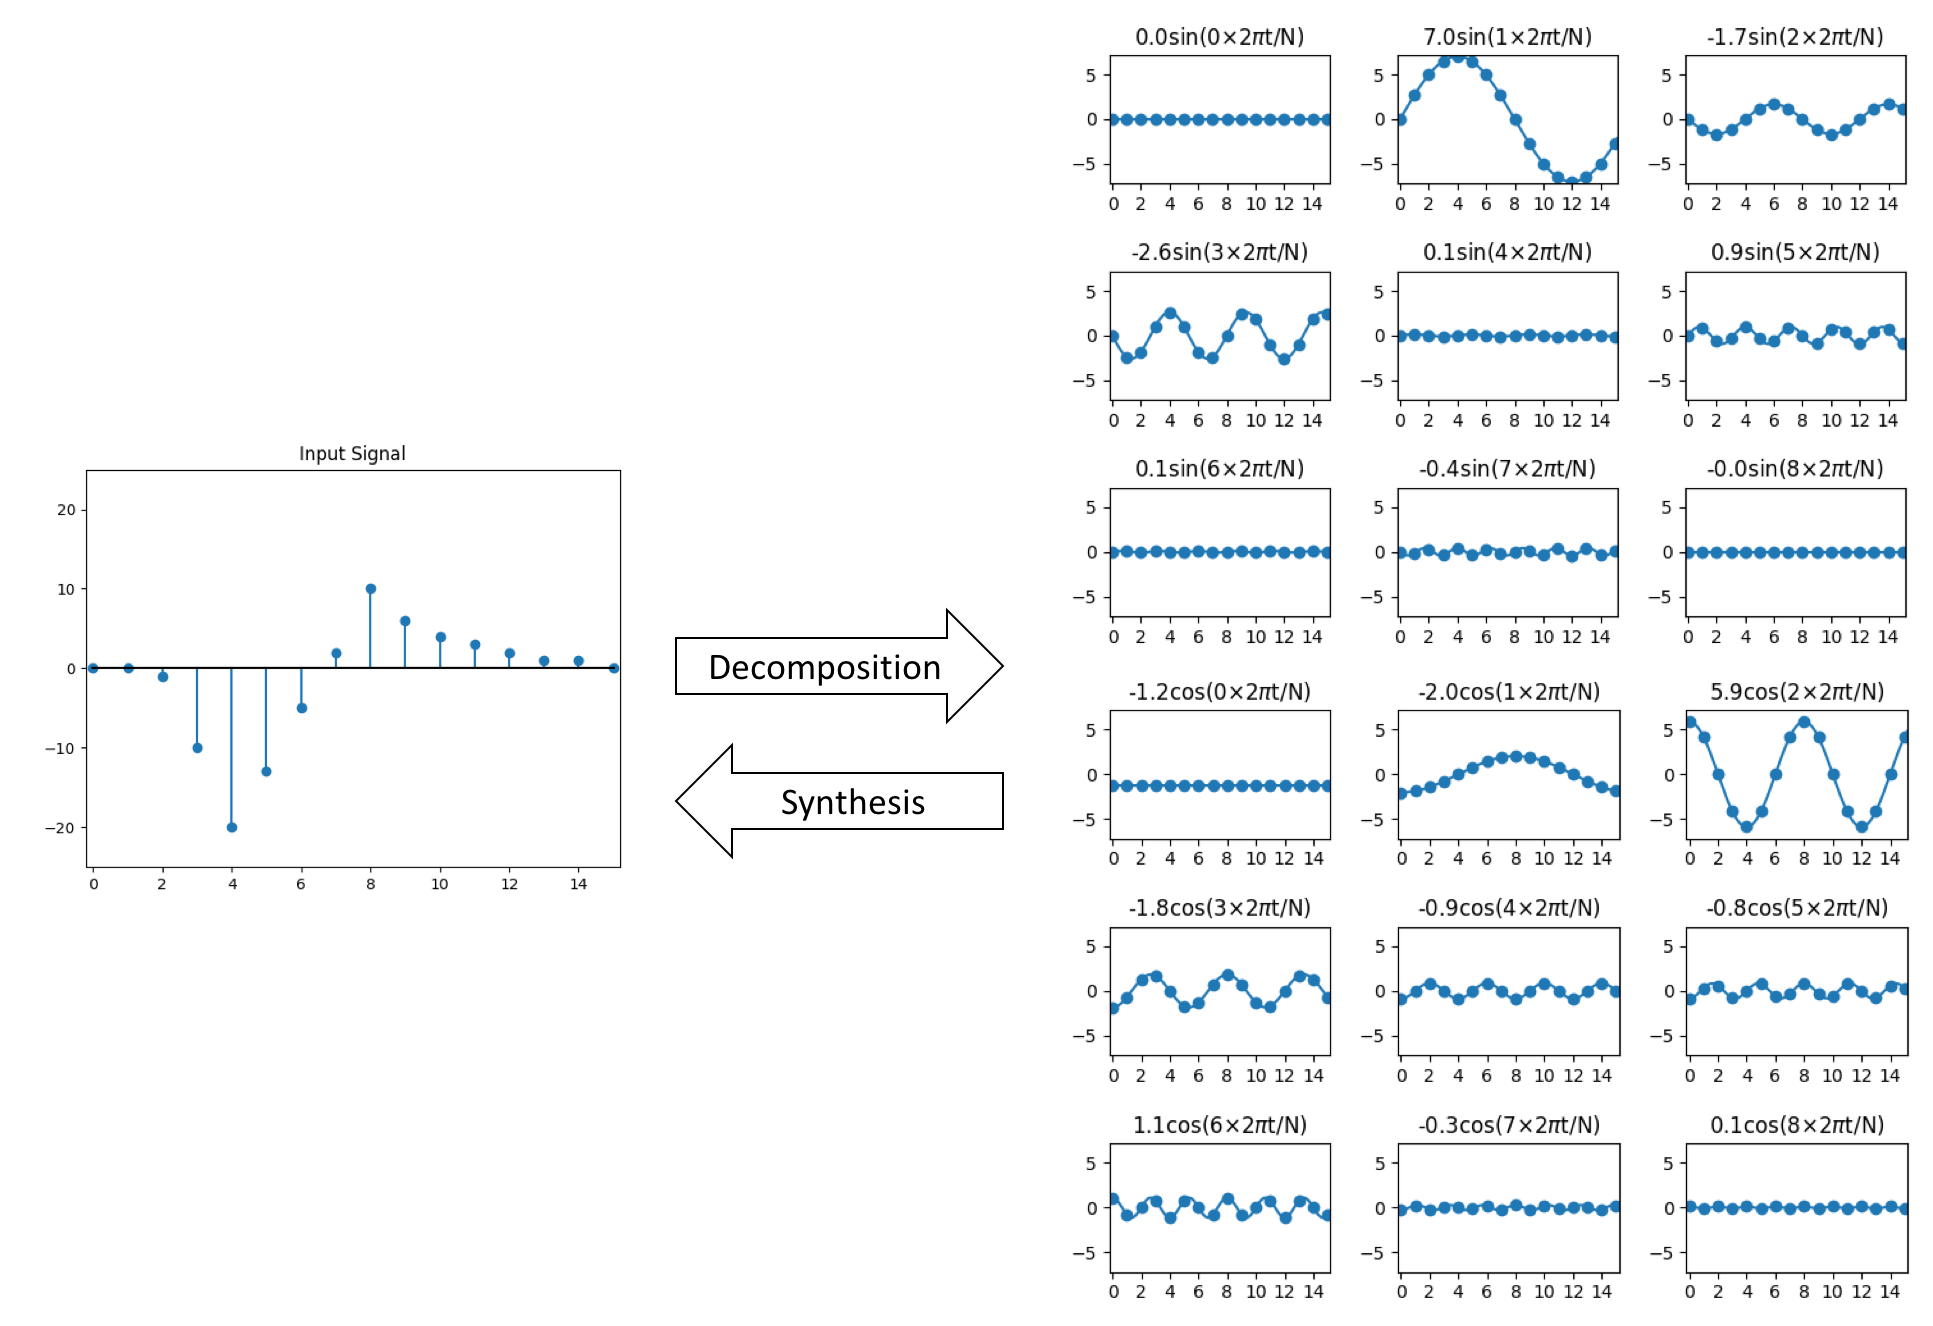
\includegraphics[width=\textwidth]{_images/DecompSynth.png}
\caption{\textbf{ Decomposition-Synthesis Relationship |} A comparison between an input signal (left) and the 18 sinusoids (right) which can be used to reconstruct the original sequence. Generally, we say that the input image can be decomposed into the 18 signals on the right and similarly that the 18 signals can be used to synthesize the original signal. (This figure was inspired by a similar figure on dspguide.com)
}\label{fig:deco}
\end{figure}

\begin{figure}
\centering
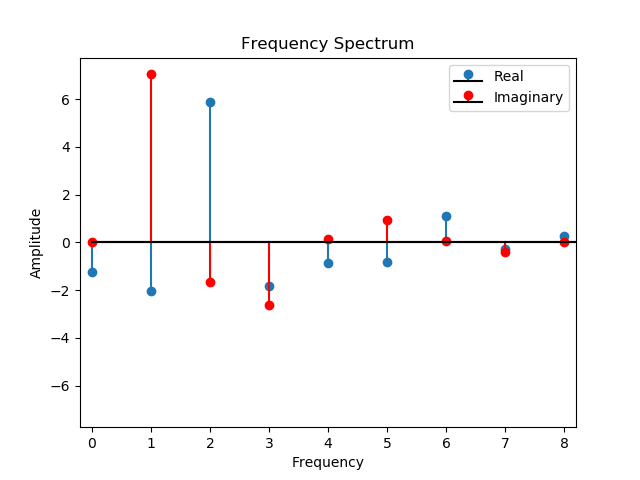
\includegraphics[width=.85\textwidth]{_images/FreqSpec.png}
\caption{\textbf{Frequency Spectrum |} In Figure \ref{fig:deco}, we decomposed a signal into 18 sines and cosines with different frequencies and amplitudes. The frequencies of these sinusoids are predetermined by the length of the input signal and the amplitudes are determined by the Fourier transform. 
}
\end{figure}


\begin{figure}
\centering
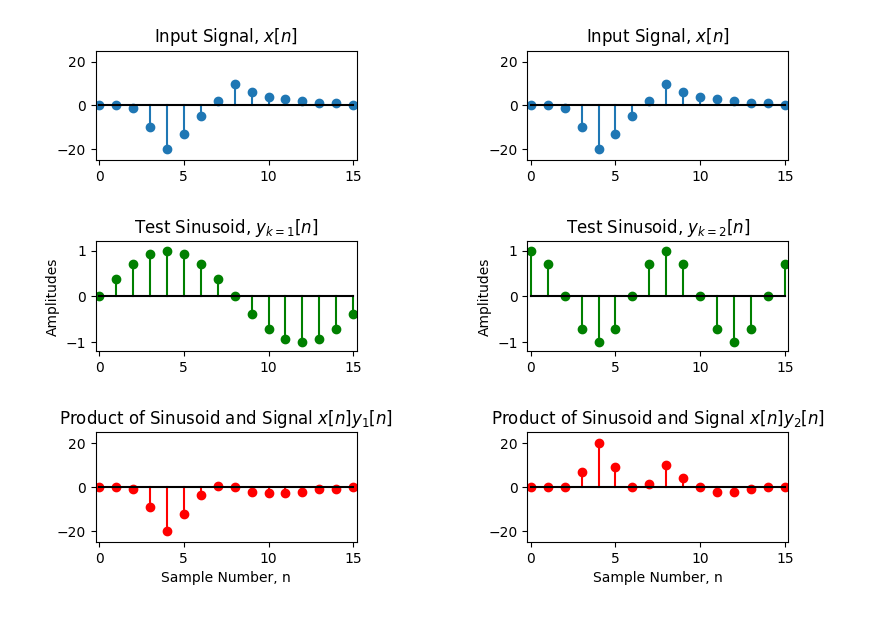
\includegraphics[width=\textwidth]{_images/FourierCorrelation3-m56p3-47p1.png}
\caption{\textbf{Correlation of an Input Signal and Two Test Sinusoids |} On the left, we show the result of correlating a particular input signal (top) with a cosine wave (middle) with period 16. For correlation, each sample in the input signal is multiplied by the corresponding sample in the test sinusoid. The result of this multiplication is shown on the bottom in red. To complete the correlation, we simply sum across all the points in the red signal. On the right, the same input signal is correlated with another cosine, this time with a period of 8. Again, the element-wise multiplication of the two signals is shown on the bottom in red. For the Fourier transform, the input signal is correlated against 16 total sinusoids (8 sines and 8 cosines).}
\end{figure}



\begin{figure}
\centering
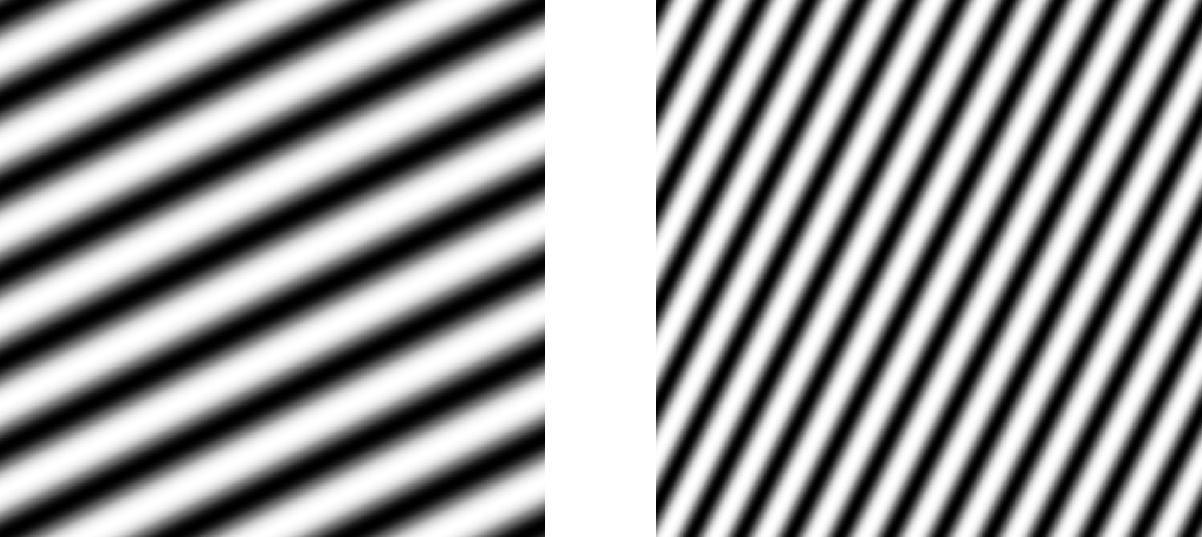
\includegraphics[width=\textwidth]{_images/TwoTestSinusoids.png}
\caption{\textbf{Examples of two-dimensional test sinusoids |} Whereas the one-dimensional Fourier transform used one-dimensional test sinusoids, the two-dimensional Fourier transform uses two-dimensional test sinusoids. Here are two potential test sinusoids that might be used on a 1024x1024 grid. While the one-dimensional Fourier transform needed N+2 sinusoids, the two-dimensional Fourier transform needs N+2xN+2 test sinusoids. Each one of these N+2xN+2 sinusoids has its own direction and frequency. As shown, the two sinusoids have different ``directions'' and frequencies. Furthermore, the sinusoids have different phases, the image on the left was generated with cosines and the image on the right was generated with sines.}
\end{figure}


\begin{figure}
\centering
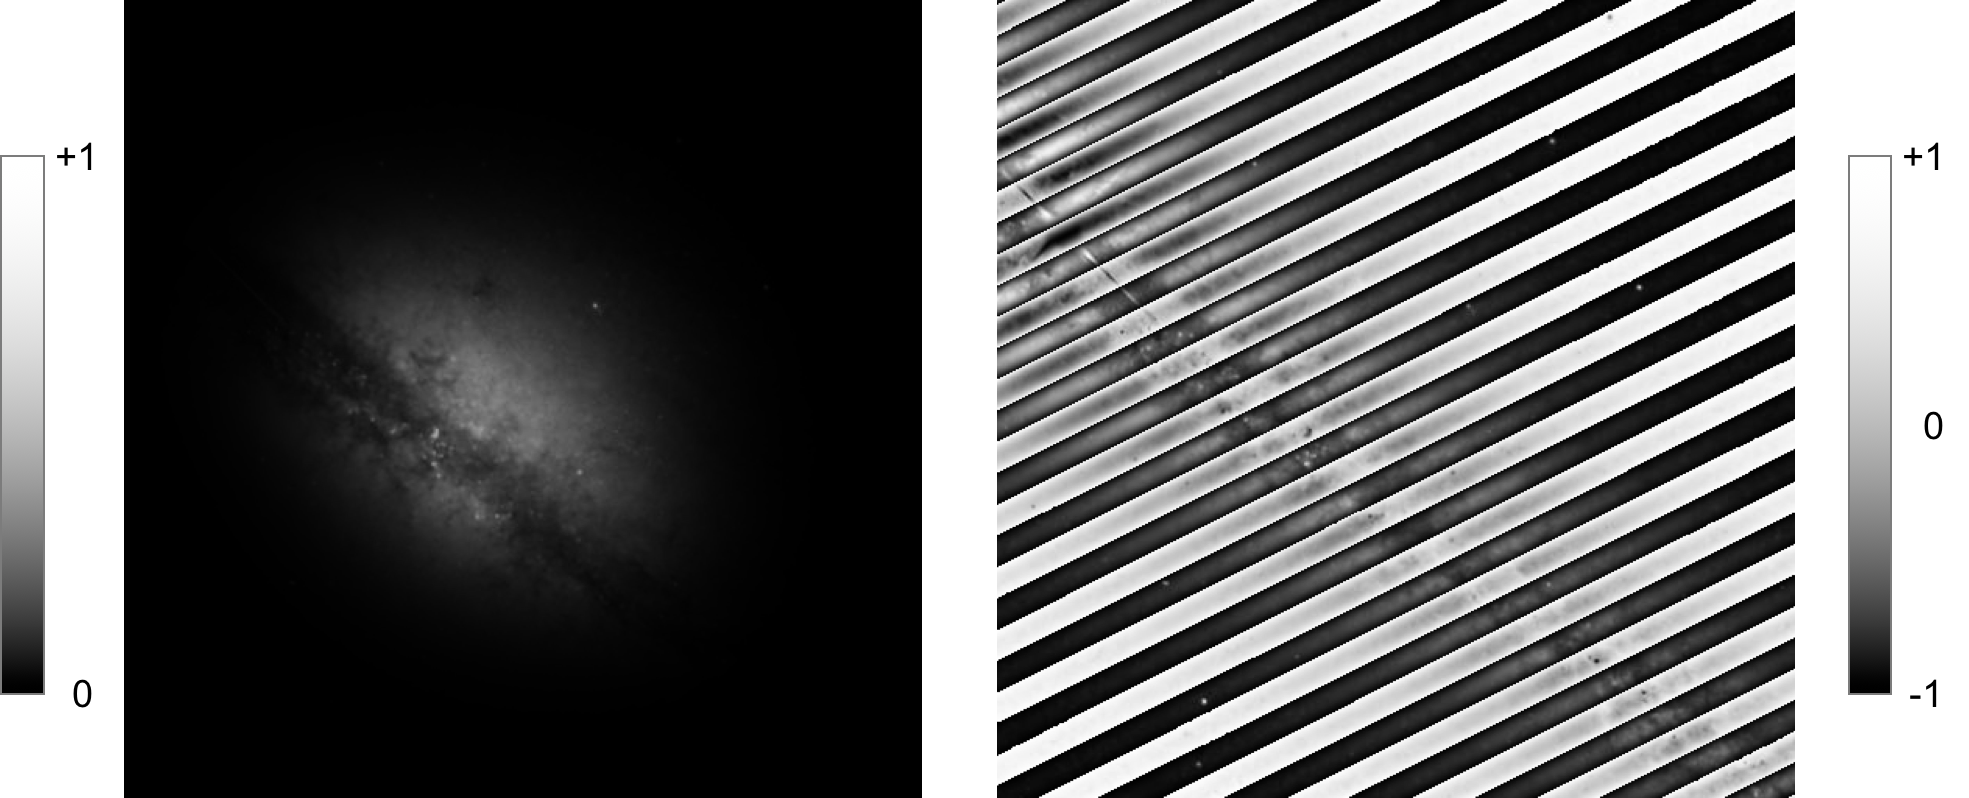
\includegraphics[width=\textwidth]{_images/ModulatedBWGalax.png}
\caption{\textbf{Demonstration of two-dimensional correlations |} On the left we have multiplied the image domain version of the galaxy in Fig. 1 by a 2D Gaussian function. On the right the same image is multipled by a 2D test sinusoid. Notice the zebra pattern that appears when the image is multiplied by the test sinusoid. This appears because the test sinusoid alternates between positive and \textit{negative} values. On the other hand, the Gaussian pattern does not take negative values and so the zebra pattern does not appear. To complete the correlation, we add together the values of every point in these two images.}
\end{figure}




\begin{figure}
\centering
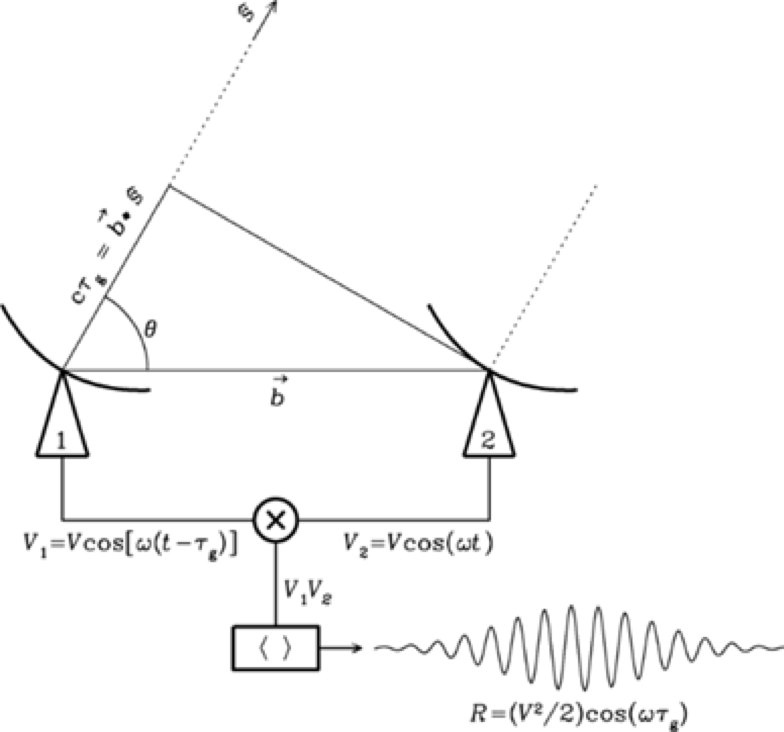
\includegraphics[width=.8\textwidth]{_images/AntGeometry.png}
\caption{\textbf{Fringe Pattern Analysis |} Schematic shows that two antennas separated by a distance $\vec{b}$ will receive time delayed versions of the same ``galactic'' signal, $V\cos(\omega t)$. If we then multiply these signals and average them over period of time, then we will obtain a signal, R, which depends on the direction of the source, $\hat{s}$, through $\tau_g$ since $\tau_g = \vec{b} \cdot \hat{s} / c$.
}
\end{figure}


\begin{figure}
\centering
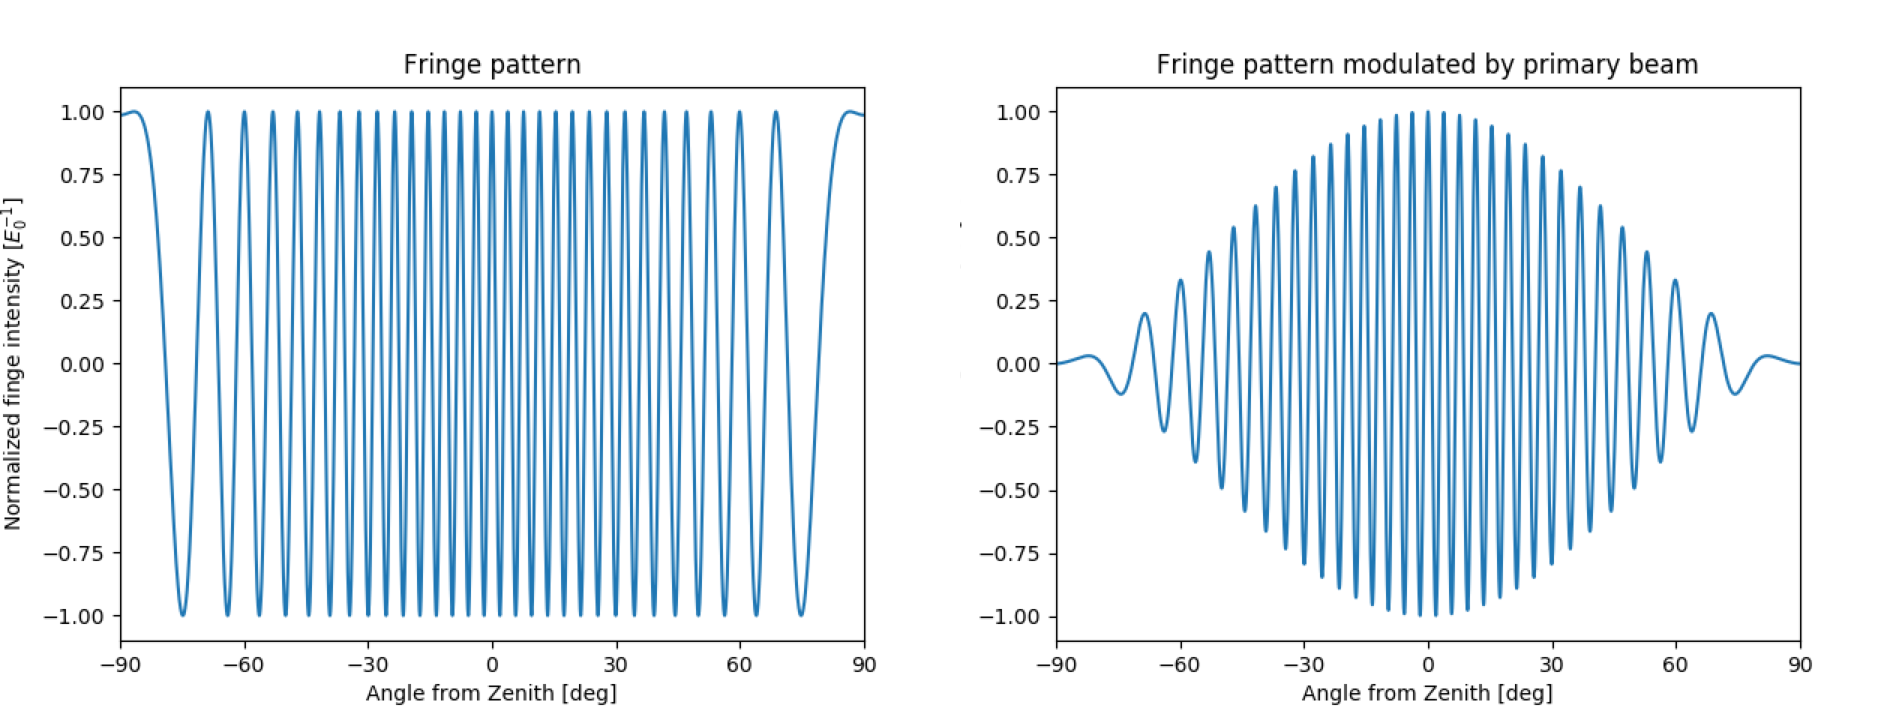
\includegraphics[width=\textwidth]{_images/FringePattern.png}
\caption{\textbf{Derived Beam Patterns |} Beam patterns for a pair of hypothetical omni-directional antennas. On the left we show the beam pattern as a function of $\theta$ and on the right, we show the same beam pattern as a function of $\cos(\theta)$. Beam patterns can be thought of as directional sensitivity patterns that describe how effectively radiation from any given direction will be picked up by the antenna. 
}
\end{figure}



\end{document}